%This is chapter 3
%%=========================================
\chapter{Use case}\label{usecase}
\section{Setup for the use case}
One example use case of the system with multiple queries and the results that can be derived from them will be discussed in this chapter. The text that will be used is \textit{The King James Version of the Bible} as found on Project Gutenberg \cite{GutenbergBible}.\\
It was chosen for two reasons:
\begin{itemize}
    \item well-known, the reader can be expected to have sufficient knowledge to follow the use case even if they have not read it in its entirety
    \item big size, analysing by hand would take considerable effort and thus using a tool such as \textbf{dragn} is preferable
\end{itemize}
I want to emphasise that while only a single text is used for this use case, achieving the result demonstrated in this chapter would be analogous for multiple texts.
The full text has been sent through the \textbf{dragn} pipeline and processed beforehand.\\
Unless otherwise specified only the 10 highest scoring relations for each relation type were included in the tables.

%
%
%------- jesus query
%
%
\clearpage
\section{Query: jesus}
\label{sec:query_jesus}
The parameters for the first query are as shown here:
\begin{itemize}
    \item Query: jesus
    \item Max nodes: 11
    \item Max edges: 300
    \item Top text samples: 100
\end{itemize}
Setting the maximum number of nodes to 11 results in a graph containing 'jesus' and ten words or phrases related in some way to 'jesus'. Setting the number of edges (also known as vertices) to a high value means all the connections will be shown. It is possible to set it to a lower value to see only the relations with the highest values if so desired.

\begin{figure}[H]
    \centering
    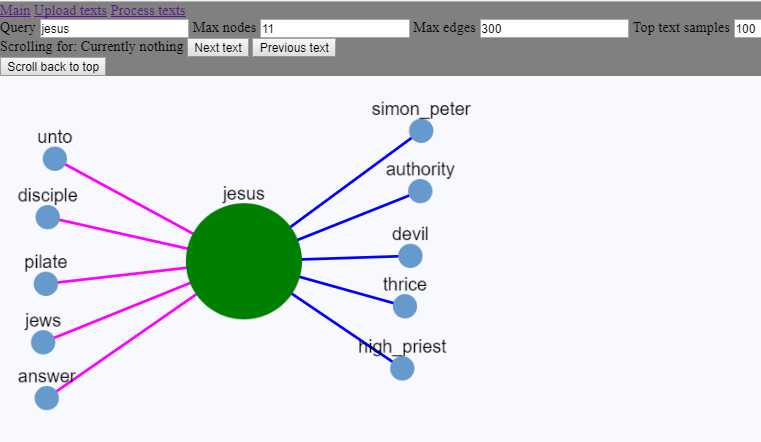
\includegraphics[scale=0.9]{fig/jesus}
    \caption{Graph for query 'jesus'}
    \label{fig:query_jesus}
\end{figure}

\clearpage
\subsection{Relations in the graph for 'jesus,'}
The following relations can be found in the result graph:
\begin{table}[H]
\centering
    \begin{tabular}{|l|l|l|}
    \hline
    subject & predicate & object \\
    \hline
    jesus &close to& simon\_peter \\
    jesus &close to& authority \\
    jesus &close to& devil \\
    jesus &close to& thrice\\
    jesus &close to& high\_priest \\
    \hline
    jesus &close to& unto\\
    jesus &close to& disciple\\
    jesus &close to& pilate\\
    jesus &close to& jews\\
    jesus &close to& answer\\
    \hline
    jesus &related to & unto\\
    jesus &related to & disciple\\
    jesus &related to & pilate\\
    jesus &related to & jews\\
    jesus &related to & answer\\
    \hline
\end{tabular}
\caption{Relations in the result graph for the query 'jesus'}
\label{tab:relations_jesus}
\end{table}

\clearpage
\subsection{Paragraphs relevant to the query 'jesus'}
The three most relevant paragraphs with their score in regards to the query are:
\blockquote{
\textbf{bible\_full.txt\_21514, 1 (Paragraph 21514 in the file)}\\
18:33 Then Pilate entered into the judgment hall again, and called Jesus, and said unto him, Art thou the King of the Jews? 18:34 Jesus answered him, Sayest thou this thing of thyself, or did others tell it thee of me? 18:35 Pilate answered, Am I a Jew? Thine own nation and the chief priests have delivered thee unto me: what hast thou done? 18:36 Jesus answered, My kingdom is not of this world: if my kingdom were of this world, then would my servants fight, that I should not be delivered to the Jews: but now is my kingdom not from hence.}
\begin{table}[H]
\centering
    \begin{tabular}{|l|l|l|l|}
    \hline
    subject & predicate & object & score \\
    \hline
    jesus & close to & pilate & 1.0\\
    jesus &close to& jews & 1.0\\
    jesus &close to& unto & 1.0\\
    jesus &close to& enter & 1.0\\
    jesus &close to& answer & 1.0\\
    jesus &close to& say & 1.0\\
    jesus &close to& world & 0.8775063207175372\\
    jesus &close to& king\_of\_jews & 0.676004216459174\\
    jesus &close to& judgement\_hall & 0.6739292059866504\\
    jesus &close to& my\_kingdom & 0.5174179934374722\\
    \hline
    jesus & related to & jews & 0.1706899529268509 \\
    jesus &related to & say & 0.09814261250477314 \\
    jesus &related to & answer & 0.034030420168504064 \\
    jesus &related to & call & 1.8997625097621448e-07 \\
    \hline
\end{tabular}
\caption{Relations found for bible\_full.txt\_21514}
\label{tab:relations_jesus_21514}
\end{table}

\clearpage
\blockquote{
\textbf{bible\_full.txt\_18763, 0.9762161536178063133580888995}\\
4:12 Now when Jesus had heard that John was cast into prison, he departed into Galilee; 4:13 And leaving Nazareth, he came and dwelt in Capernaum, which is upon the sea coast, in the borders of Zabulon and Nephthalim: 4:14 That it might be fulfilled which was spoken by Esaias the prophet, saying, 4:15 The land of Zabulon, and the land of Nephthalim, by the way of the sea, beyond Jordan, Galilee of the Gentiles; 4:16 The people which sat in darkness saw great light; and to them which sat in the region and shadow of death light is sprung up.}
\begin{table}[H]
\centering
    \begin{tabular}{|l|l|l|l|}
    \hline
    subject & predicate & object & score \\
    \hline
    jesus &close to & galilee & 1.0\\
    jesus &close to& nazareth & 1.0\\
    jesus &close to& john & 1.0\\
    jesus &close to& saw & 1.0\\
    jesus &close to& sit & 1.0\\
    jesus &close to& say & 1.0\\
    jesus &close to& depart & 1.0\\
    jesus &close to& capernaum & 0.8716620885947697\\
    jesus &close to& fulfill & 0.8598812801210459\\
    jesus &close to& dwelt\_in\_capernaum & 0.2627662846808881\\
    \hline
    jesus & related to & john & 0.19577093636686257 \\
    jesus &related to & galilee & 0.1565230454832303 \\
    jesus &related to & nazareth & 0.11995120425385629 \\
    jesus &related to & depart & 0.11585843258452326 \\
    jesus &related to & say & 0.11561349559243331 \\
    jesus &related to & saw & 0.11249972841114071 \\
    \hline
\end{tabular}
\caption{Relations found for bible\_full.txt\_18763}
\label{tab:relations_jesus_18763}
\end{table}

\clearpage
\blockquote{\textbf{bible\_full.txt\_18947, 0.9337834238561429497345759280}\\
11:2 Now when John had heard in the prison the works of Christ, he sent two of his disciples, 11:3 And said unto him, Art thou he that should come, or do we look for another? 11:4 Jesus answered and said unto them, Go and shew John again those things which ye do hear and see: 11:5 The blind receive their sight, and the lame walk, the lepers are cleansed, and the deaf hear, the dead are raised up, and the poor have the gospel preached to them.}
\begin{table}[H]
\centering
    \begin{tabular}{|l|l|l|l|}
    \hline
    subject & predicate & object & score \\
    \hline
    jesus &close to & raise & 1.0\\
    jesus &close to& disciple & 1.0\\
    jesus &close to& preach & 1.0\\
    jesus &close to& say & 1.0\\
    jesus &close to& answer & 1.0\\
    jesus &close to& unto & 1.0\\
    jesus &close to& gospel & 0.7220483212774963\\
    jesus &close to& john & 0.6948157183491428\\
    jesus &close to& receive & 0.31074260643649365\\
    jesus &close to& deaf\_dead & 0.2668806801251524\\
    \hline
    jesus & related to & answer & 0.1307478787056254 \\
    jesus &related to & say & 0.12355058556155199 \\
    jesus &related to & kingdom\_of\_god & 0.09684031278231553 \\
    jesus &related to & suppose & 0.0777098842002729 \\
    jesus &related to & disciple & 0.06644093989493592 \\
    jesus &related to & receive & 0.027963657641532764 \\
    jesus &related to & come & 1.9729556723760588e-07 \\
    \hline
\end{tabular}
\caption{Relations found for bible\_full.txt\_18947}
\label{tab:relations_jesus_18947}
\end{table}

\clearpage
\subsection{Analysis of the query 'jesus'}
\label{subsec:interpretation_jesus}
A simple one-word query will produce a graph with words or phrases that co-occur either directly with the word from the query or that co-occur with the same words as discussed in \ref{sec:kbcompute} and \ref{sec:popdict}.\\
As such, it is not unexpected that the result graph shows that \textit{Jesus} often co-occurs with a disciple of his, \textit{Simon Peter} or the man responsible for making him a martyr, \textit{Pilate} as both seen in \ref{tab:relations_jesus} and another of his disciples, John, as we can see in table \ref{tab:relations_jesus_18763}. In the same table we can see that the highest scoring of the Cosine Similarity relations (related to) is the one with John; indicating that 'John' and 'Jesus' have a high similarity. Further the expected connections between his preachings and the audience thereof can be found in the highest scoring paragraph, as seen in table \ref{tab:relations_jesus_21514}: \textit{jesus close to jews}, \textit{jesus close to king\_of\_jews}, \textit{jesus close to preach}. Jesus had a strong connection to Jews and was known for his preachings. The result graph emphasises this connection and lets the user gain information about Jesus and what he did without reading a single page of the bible. Of course such an analysis is very superficial, but that is a given considering the nature of Distant Reading.\\
Especially interesting is paragraph 21514 (\ref{tab:relations_jesus_21514}). In it, Jesus has a conversation with Pilate, the man who would later sentence him to be crucified. In the conversation, Jesus indicates that he is the servant of heaven: \blockquote{\textit{My kingdom is not of this world}}. This short paragraph captures the spirit of Jesus relatively well, essential information about him is contained therein. His celestial nature is further extrapolated by the second-highest scoring paragraph: \blockquote{\textit{The people which sat in darkness saw great light; and to them which sat in the region and shadow of death light is sprung up.}} and the third-highest scoring paragraph, where Jesus talks about the miracles he performed: \blockquote{\textit{Go and shew John again those things which ye do hear and see:  [...] The blind receive their sight,  and the lame walk, the lepers are cleansed, and the deaf hear, the dead are raised up}}.\\
The appearance of 'devil' in the result graph may be unexpected at first and indicate an unexpected connection between Jesus and the Devil. Most likely the connection stems from the passages of the bible where the Devil tempts Jesus. 'Devil' is absent from the highest scoring paragraphs because the relation between 'Jesus' and 'Devil' is not strong enough to score the paragraphs containing it high enough. To further explore the aforementioned link of the relation 'jesus close to devil' we can see in the graph \ref{fig:query_jesus} we can perform a second query: 'jesus,devil'.

%
%
%------------ jesus, devil query
%
%
\clearpage
\section{Query: jesus, devil}
\label{sec:query_jesus,devil}
The parameters for the first query are as shown here:
\begin{itemize}
    \item Query: jesus,devil
    \item Max nodes: 11
    \item Max edges: 300
    \item Top text samples: 100
\end{itemize}

\begin{figure}[H]
    \centering
    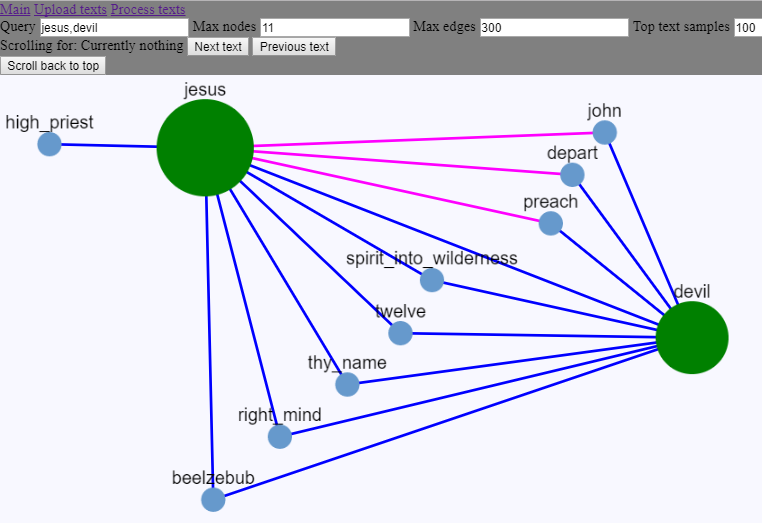
\includegraphics[scale=0.9]{fig/jesus,devil}
    \caption{Graph for query 'jesus,devil'}
    \label{fig:query_jesus,devil}
\end{figure}

\clearpage
\subsection{Relations in the graph for 'jesus,devil'}
The following relations can be found in the result graph:
\begin{table}[H]
\centering
    \begin{tabular}{|l|l|l|}
    \hline
    subject & predicate & object \\
    \hline
    jesus &close to& high\_priest \\
    jesus &close to& beelzebub \\
    jesus &close to& right\_mind \\
    jesus &close to& thy\_name\\
    jesus &close to& twelve \\
    \hline
    jesus &close to& spirit\_into\_wilderness\\
    jesus &close to& devil\\
    jesus &close to& preach\\
    jesus &close to& depart\\
    jesus &close to& john\\
    \hline
    jesus &related to & preach\\
    jesus &related to & depart\\
    jesus &related to & john\\
    jesus &related to & jews\\
    jesus &related to & answer\\
    \hline
    devil &close to& beelzebub \\
    devil &close to& right\_mind \\
    devil &close to& thy\_name \\
    devil &close to& twelve\\
    devil &close to& spirit\_into\_wilderness \\
    \hline
    devil &close to& jesus\\
    devil &close to& preach\\
    devil &close to& depart\\
    devil &close to& john\\
    \hline
    devil &related to & preach\\
    devil &related to & depart\\
    devil &related to & john\\
    \hline
\end{tabular}
\caption{Relations in the result graph for the query 'jesus,devil'}
\label{tab:relations_jesus,devil}
\end{table}

\clearpage
\subsection{Paragraphs relevant to the query 'jesus,devil'}
\blockquote{
\textbf{bible\_full.txt\_18763, 1}\\
4:12 Now when Jesus had heard that John was cast into prison, he departed into Galilee; 4:13 And leaving Nazareth, he came and dwelt in Capernaum, which is upon the sea coast, in the borders of Zabulon and Nephthalim: 4:14 That it might be fulfilled which was spoken by Esaias the prophet, saying, 4:15 The land of Zabulon, and the land of Nephthalim, by the way of the sea, beyond Jordan, Galilee of the Gentiles; 4:16 The people which sat in darkness saw great light; and to them which sat in the region and shadow of death light is sprung up.}
\label{quote:jesus_devil_18763}
\begin{table}[H]
\centering
    \begin{tabular}{|l|l|l|l|}
    \hline
    subject & predicate & object & score \\
    \hline
    jesus & close to & depart & 1.0\\
    jesus &close to& say & 1.0\\
    jesus &close to& sit & 1.0\\
    jesus &close to& nazareth & 1.0\\
    jesus &close to& john & 1.0\\
    jesus &close to& galilee & 1.0\\
    jesus &close to& saw & 0.8775063207175372\\
    jesus &close to& capernaum & 0.8716620885947697\\
    jesus &close to& fulfill & 	0.8598812801210459\\
    jesus &close to& zabulon\_nephthalim & 0.2627662846808881\\
    \hline
    jesus & related to & john & 0.19577093636686257 \\
    jesus &related to & galilee & 0.1565230454832303 \\
    jesus &related to & nazareth & 0.11995120425385629 \\
    jesus &related to & depart & 0.11585843258452326 \\
    jesus &related to & say & 	0.11561349559243331 \\
    jesus &related to & saw & 	0.11249972841114071 \\
    \hline
\end{tabular}
\caption{Relations found for bible\_full.txt\_18763}
\label{tab:relations_jesus,devil_18763}
\end{table}

\clearpage
\textbf{bible\_full.txt\_19624, 0.9980094901993289666129572101}\\
\blockquote{
5:15 And they come to Jesus, and see him that was possessed with the devil, and had the legion, sitting, and clothed, and in his right mind: and they were afraid.}
\begin{table}[H]
\centering
    \begin{tabular}{|l|l|l|l|}
    \hline
    subject & predicate & object & score \\
    \hline
    jesus & close to & devil & 1.0\\
    jesus &close to& sit & 1.0\\
    jesus &close to& right\_mind &0.7637623651652926\\
    jesus &close to& legion & 0.581402615101797\\
    jesus &close to& afraid & 0.08126797684445049\\
    \hline
    devil &close to& possess & 1.0\\
    devil &close to& right\_mind & 1.0\\
    devil &close to& clothe &	0.522321459997405\\
    devil &close to& legion & 0.513647727750805\\
    devil &close to& afraid & 0.14408345959927174\\
    \hline
    jesus & related to & unto & 0.09325454471923895 \\
    jesus &related to & come & 1.9729556723760588e-07 \\
    \hline
\end{tabular}
\caption{Relations found for bible\_full.txt\_19624}
\label{tab:relations_jesus,devil_19624}
\end{table}

\clearpage
\blockquote{
\textbf{bible\_full.txt\_18947, 0.9908170021801287219957252699}\\
11:2 Now when John had heard in the prison the works of Christ, he sent two of his disciples, 11:3 And said unto him, Art thou he that should come, or do we look for another? 11:4 Jesus answered and said unto them, Go and shew John again those things which ye do hear and see: 11:5 The blind receive their sight, and the lame walk, the lepers are cleansed, and the deaf hear, the dead are raised up, and the poor have the gospel preached to them.}
\begin{table}[H]
\centering
    \begin{tabular}{|l|l|l|l|}
    \hline
    subject & predicate & object & score \\
    \hline
    jesus & close to & preach & 1.0\\
    jesus &close to& disciple & 1.0\\
    jesus &close to& say  &0.7637623651652926\\
    jesus &close to& unto & 0.581402615101797\\
    jesus &close to& answer & 0.08126797684445049\\
    jesus &close to& gospel & 0.7220483212774963\\
    jesus &close to& john &0.6948157183491428\\
    jesus &close to& receive & 0.31074260643649365\\
    jesus &close to& deaf\_dead & 0.2668806801251524\\
    jesus &close to& lame\_walk\_leper & 0.2668806801251524\\
    \hline
    jesus & related to & answer & 0.1307478787056254 \\
    jesus &related to & say & 0.12355058556155199 \\
    jesus & related to & unto & 	0.10397979732017294 \\
    jesus &related to & kingdom\_of\_god & 	0.09684031278231553 \\
    jesus & related to & suppose & 0.0777098842002729 \\
    jesus &related to & disciple & 0.06644093989493592\\
    jesus & related to & receive & 0.027963657641532764 \\
    jesus &related to & come & 1.9729556723760588e-07 \\
    \hline
\end{tabular}
\caption{Relations found for bible\_full.txt\_18947}
\label{tab:relations_jesus,devil_18497}
\end{table}

\clearpage
\subsection{Analysis of the query 'jesus,devil'}
\label{subsec:analysis_jesus,devil}
As we can see, 'bible\_full.txt\_18763', \ref{quote:jesus_devil_18763}, has a higher score for this query than for the previous one. This simply means that for the second query 'devil' has a relation with at least one of the phrases occurring in this paragraph. The relation does not have to occur in that particular paragraph for it to play a role in the score, 'devil close to / related to some-phrase-in-the-paragraph' increases the score for that particular paragraph. In the case of the two queries explored thus far, it is enough to boost the score over the query for just 'jesus'.\\
Further of note is the size of the nodes for 'jesus' and 'devil': A bigger size means that the node's relations have overall higher values, thus the relations containing 'jesus' have, on average, a higher score than the ones containing 'devil'.\\
To showcase the actual distant reading capabilities of \textbf{dragn}, all texts containing 'devil' that were relevant to the query will now be examined. Doing so is simple, simply select the option from the context menu for 'devil'. The first three found paragraphs are as follows:
\blockquote{
\textbf{bible\_full.txt\_19138, 0.7504529032262834051903739287}\\
17:18 And Jesus rebuked the devil; and he departed out of him: and the child was cured from that very hour.}
\blockquote{
\textbf{bible\_full.txt\_20138, 0.743060272861912940301581312}\\
4:1 And Jesus being full of the Holy Ghost returned from Jordan, and was led by the Spirit into the wilderness, 4:2 Being forty days tempted of the devil. And in those days he did eat nothing: and when they were ended, he afterward hungered.}
\blockquote{
\textbf{bible\_full.txt\_18754, 0.6234419471291024632964296787}\\
4:1 Then was Jesus led up of the spirit into the wilderness to be tempted of the devil.}
The paragraphs shown here are the first three containing the word 'devil' in the result for the query 'jesus,devil'.\\
Using the context reader it is to possible to gain further context for the passages. It allows reading the text passages before and after a given paragraph, thus allowing the reader to gain additional understanding by reading only a few paragraphs as opposed to reading the entire book.\\
Reading the paragraphs before 19138 lets the reader find mention of a character named 'Elias':
\blockquote{
\textbf{bible\_full.txt\_19133}\\
17:12 But I say unto you, That \textbf{Elias} is come already, and they knew him not, but have done unto him whatsoever they listed. Likewise shall also the Son of man suffer of them.}
Now the analysis in section \ref{subsec:interpretation_jesus} can be continued. As expected, the connection between Jesus and the Devil is not an unexpected one, Jesus exorcises a demon, referred to as 'devil' in paragraph 19138, comes face to face with a demon (referred to as 'devil') in \ref{tab:relations_jesus,devil_19624}, and is tempted while meditating or praying in the wilderness. The found paragraphs contain interactions between Jesus and the Devil; paragraphs that would be hard to find by hand without the assistance of a tool. \textbf{dragn} gives the reader additional understanding of the paragraphs by allowing the user to read previous and following text passages. Thus additional context and understanding of the bible passages can be gained without reading them in their entirety.\\
Finding the passages in the bible containing both characters was made very easy as well, a task which would took significant effort otherwise.\\
Unclear phrases or words can be added to the query to get information about them the same way was done with 'Jesus'.\\
One such case will be examined using the name 'Elias': Who is Elias and what is his relation to Jesus? Is there a connection between Elias, Jesus and the Devil? Instead of reading further paragraphs, the user can utilise \textbf{dragn} to get an overview of that character and his relation to Jesus.

%
%
%------------ jesus,elias query
%
%
\clearpage
\section{Query: jesus,elias}
\label{sec:query_jesus,elias}
\begin{itemize}
    \item Query: jesus,elias
    \item Max nodes: 11
    \item Max edges: 300
    \item Top text samples: 100
\end{itemize}
\begin{figure}[H]
    \centering
    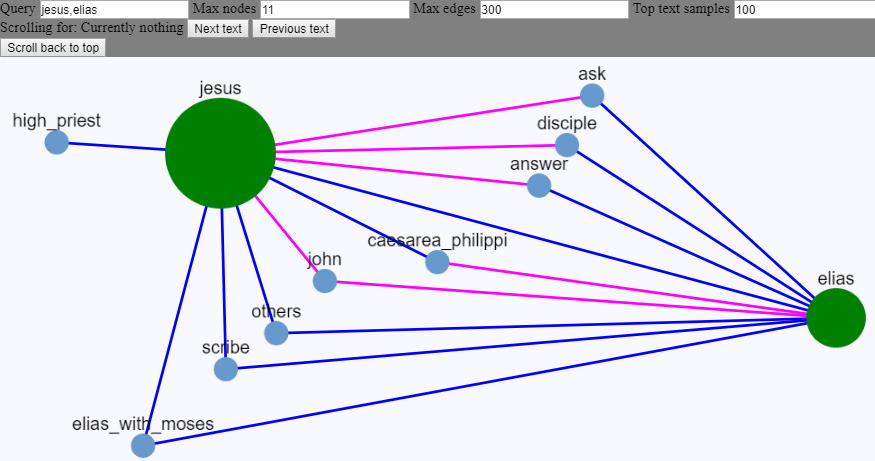
\includegraphics[scale=0.8]{fig/jesus,elias}
    \caption{Graph for query 'jesus,elias'}
        \label{fig:query_jesus,elias}
\end{figure}

\clearpage
\subsection{Paragraphs relevant to the query 'jesus,elias'}
\label{subsec:jesuselias}
As the goal of this query is to specifically find the relation between Jesus and Elias, and to understand who Elias is and what he does, the relations in the paragraphs are omitted. The three highest scoring paragraphs are:
\blockquote{
\textbf{bible\_full.txt\_19741, 1}\\
8:27 And Jesus went out, and his disciples, into the towns of Caesarea Philippi: and by the way he asked his disciples, saying unto them, Whom do men say that I am? 8:28 And they answered, John the Baptist; but some say, Elias; and others, One of the prophets.}
\blockquote{
\textbf{bible\_full.txt\_19111, 0.7760642136698343241237380147}\\
16:13 When Jesus came into the coasts of Caesarea Philippi, he asked his disciples, saying, Whom do men say that I the Son of man am? 16:14 And they said, Some say that thou art John the Baptist: some, Elias; and others, Jeremias, or one of the prophets.}
\blockquote{
\textbf{bible\_full.txt\_19132, 0.7717350897508739809379502151}\\
17:10 And his disciples asked him, saying, Why then say the scribes that Elias must first come? 17:11 And Jesus answered and said unto them, Elias truly shall first come, and restore all things.}

\subsection{Analysis of the query 'jesus,elias'}
It becomes obvious that Jesus holds Elias in high regard and that Elias is a person of importance, as indicated by him saying that 'Elias truly shall first come, and restore all things' (Paragraph 19132). The result however does not easily reveal the nature of Elias; his profession or importance in more detail. The query being 'jesus,elias' most likely causes Jesus to overshadow Elias and thus the paragraphs that focus solely on Elias are scored lower. To fix that, a simple query of 'elias' can be performed.

%
%
%------------ elias query
%
%
\clearpage
\section{Query: 'elias'}
\label{sec:query_elias}
\begin{itemize}
    \item Query: 'elias'
    \item Max nodes: 21
    \item Max edges: 300
    \item Top text samples: 100
\end{itemize}
\begin{figure}[H]
    \centering
    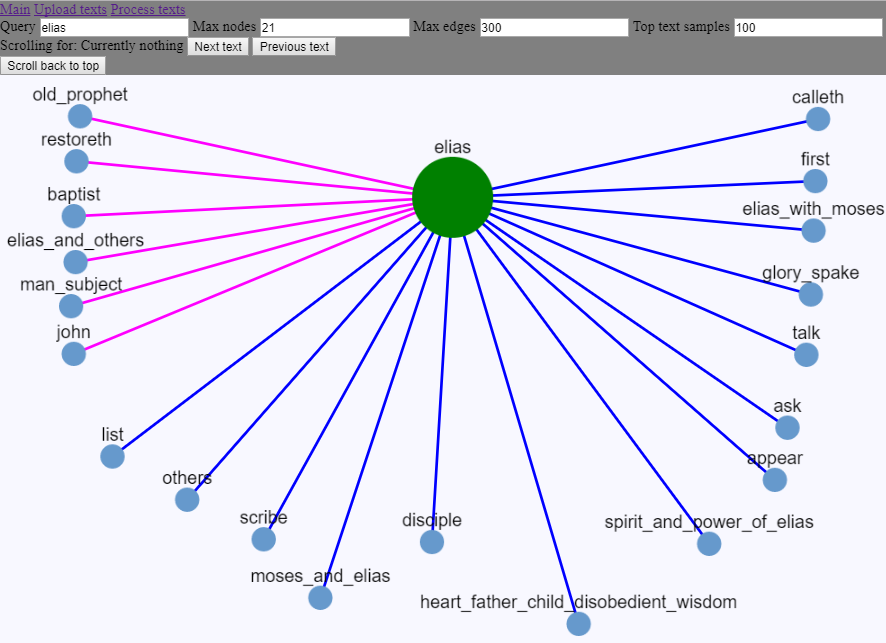
\includegraphics[scale=0.8]{fig/elias}
    \caption{Graph for query 'elias'}
    \label{fig:query_elias}
\end{figure}

\clearpage
\subsection{Analysis of the result for query 'elias'}
Again the paragraphs from \ref{subsec:jesuselias} containing 'Jesus' and 'Elias' are found. A quick glance over the found paragraphs shows that Elias is often mentioned together with Jesus and rarely alone. However, among the result one particular paragraph can be found:
\blockquote{
\textbf{bible\_full.txt\_24032, 0.1747682234100624985942175979}\\
5:17 Elias was a man subject to like passions as we are, and he prayed earnestly that it might not rain: and it rained not on the earth by the space of three years and six months.}
By reading the previous paragraph it becomes clear Elias is used solely as the example of a very faithful man:

\blockquote{
5:16 Confess your faults one to another, and pray one for another, that ye may be healed. The effectual fervent prayer of a righteous man availeth much.\\
5:17 Elias was a man subject to like passions as we are, and he prayed earnestly that it might not rain: and it rained not on the earth by the space of three years and six months.\\
5:18 And he prayed again, and the heaven gave rain, and the earth brought forth her fruit.\\
5:19 Brethren, if any of you do err from the truth, and one convert him; 5:20 Let him know, that he which converteth the sinner from the error of his way shall save a soul from death, and shall hide a multitude of sins.
}
So faithful, that his prayers influence the weather on a global scale. Using that information, we can better understand the passage found for the query 'jesus,devil' (\ref{subsec:analysis_jesus,devil}) and 'jesus,elias' (\ref{subsec:jesuselias}). The assumption can be made that Elias is mentioned as an example of a person with strong faith, a positive example that others shall follow. This additional information was not immediately clear when just reading the paragraphs on their own without the assistance of \textbf{dragn}.

\section{Summary of the use case}
Using \textbf{dragn} it was possible to gain a rudimentary understanding of 'Jesus', as seen in \ref{sec:query_jesus}. While a full analysis is neither possible nor intended, we were able to ascertain certain aspects of his character. Connections between Jesus and Jews were found, as were connections to his celestial nature \ref{subsec:interpretation_jesus}. An unexpected connection between Jesus and the Devil could be checked \ref{sec:query_jesus,devil} and paragraphs describing their interactions were found. Both of those tasks would have taken a considerable amount of time when doing by hand or even using tools not designed for the task of Distant Reading, such as a basic search interface. Further, using the context reader it was possible to read passages before and after the paragraphs found as a result of the query \ref{subsec:analysis_jesus,devil} which lead us to find mention of a certain character named 'Elias'. Attempting to find a link between Jesus and Elias lead us to find paragraphs in which Jesus was either mistaken for Elias, or in which it seemed that Jesus held Elias in high regards and considered him a person of importance \ref{sec:query_jesus,elias}. It did not become apparent who Elias is or what he did to make him so noteworthy. Reading the result paragraphs for the query 'elias' however revealed that Elias became known for having faith strong enough to cause droughts or rain on a global scale \ref{sec:query_elias}. Thus the mentions of Elias gained additional context: Elias was most likely used as a positive example, a person of strong faith, an example to follow. Using the \textbf{dragn} search interface it was possible to gain a basic understanding of Jesus, his connection and interactions to the Devil and who this 'Elias' person is and what he did, in a quick, direct and logical way, using Distant Reading and nodes in a graph.